We first import the dataset and encode each categorical feature using \textit{one-hot encoding}. This means that numerical features will be left unchanged while for each categorical feature the process is the following:
\begin{description}
    \item[1.] Determine all the distinct values of that feature (categories)
    \item[2.] For each category generate a new binary column
    \item[3.] Assign values to the binary columns according to categories featred in each line.   
\end{description}
\begin{center}
    \begin{tabular}{|c|}
        \hline
        feature \\
        \hline
        \hline
        category 1 \\
        \hline
        category 2 \\
        \hline
        category 3 \\
        \hline
        category 2 \\
        \hline
    \end{tabular}
    \quad
    \begin{tabular}{|c|c|c|}
        \hline
        category 1 & category 2 & category 3\\
        \hline
        \hline
        1 & 0 & 0 \\
        \hline
        0 & 1 & 0 \\
        \hline 
        0 & 0 & 1 \\
        \hline
        0 & 1 & 0 \\
        \hline
    \end{tabular}    
\end{center}
\begin{lstlisting}[language=Python, caption= Data encoding]
    import pandas as pd

    df = pd.read_csv('Data/bank/bank-additional-full.csv', sep=';')
    display(df.head())
    cat_col = df.dtypes=='O'
    df_enc = pd.get_dummies(df.loc[:, cat_col], prefix=df.columns[cat_col])
    df_enc = df_enc.join(df.loc[:, np.logical_not(cat_col)])

    df_enc = df_enc.drop('y_no', axis=1) #deleting column since attribute "y" is binary
    df_enc = df_enc.drop('duration', axis = 1) #drop the duration column (see attribute information)

\end{lstlisting}

\subsection{Data Exploration}
Independently from encoding we can also perform some data exploration, in order to gain useful insights about some of the attributes featured in the dataset. There are 11 categorical features and the remaining are numerical. Categorical data will be explored by means of \textit{pie charts} while numerical data will be explored by means of a \textit{scatterplot matrix}

\begin{figure}[H]
    \centering
    \subfloat[1][caption1]{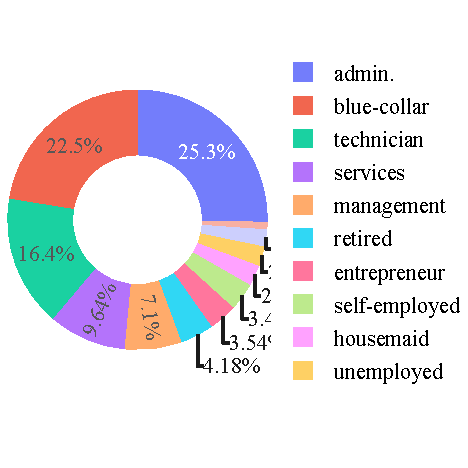
\includegraphics[scale = 0.7]{pictures/pieplotjob.pdf}}
    \qquad
    \qquad
    \subfloat[2][caption2]{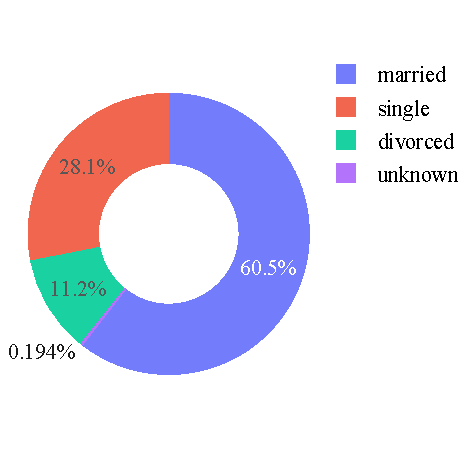
\includegraphics[scale = 0.7]{pictures/pieplotmarital.pdf}}
   
\end{figure}



